\begin{abstract}
In this project we will be writing a molecular dynamics program in \texttt{C++} that models the behaviour of a system of Argon atoms, and use the program to study statistical properties of the system. We will do measurements of temperature, pressure and diffusion. We will be using the Lennard-Jones potential to model the interatomic interactions, and the Verlet algorithm for integrating the particle motion. An important part of the project is converting all the constants and variables used in the program to so-called Molecular Dynamics units. In the end we will implement the Berendsen thermostat in our code.
\end{abstract}

\begin{figure}[ht!]
    \centering
    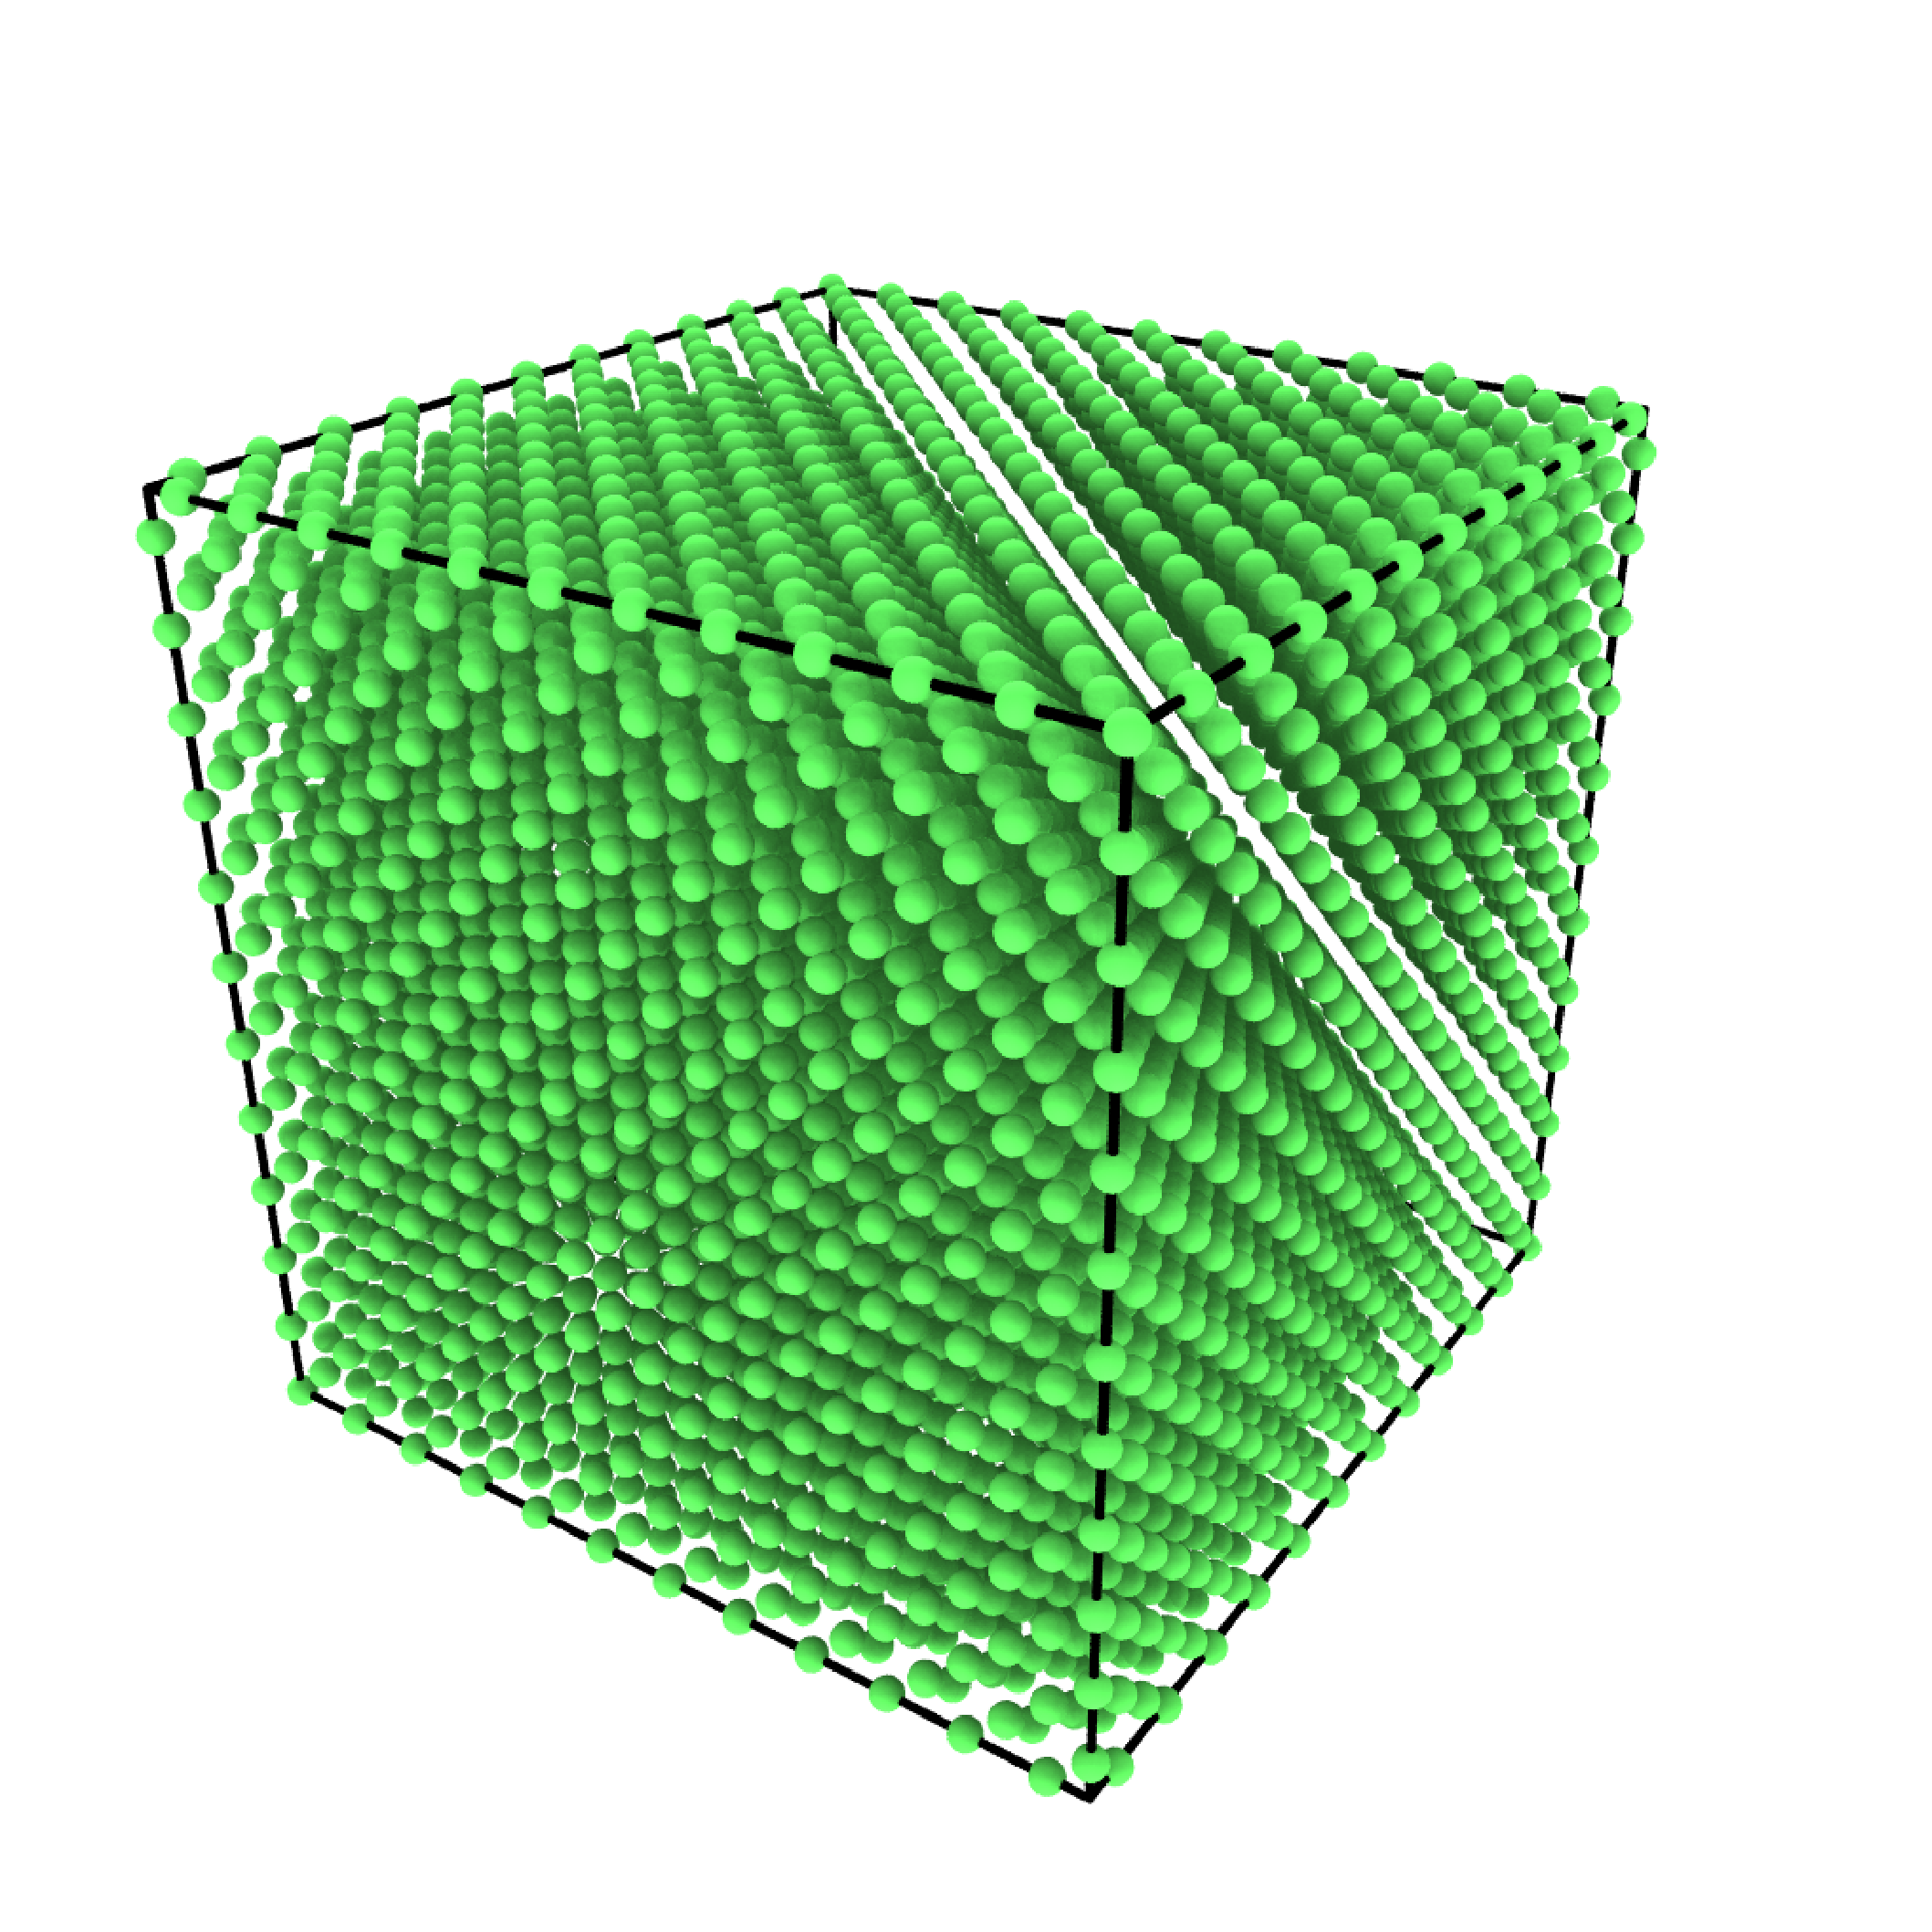
\includegraphics[width =.80\textwidth]{bilder/fcc.eps}
    \parbox{4in} {
        \caption{
            \small{
                Visualization of a 12x12x12 Argon system of fcc unit cells with $a = 5.260$ \AA.
            }
            \label{fig:fcc}
        }
    }
\end{figure}

\subsection*{Total energy}
We find the total internal energy of the system using the Lennard-Jones potential and the standard equation for kinetic energy (see Appendix for derivations of dimensionless versions of these equations). Using that we can plot the the total internal energy as a function of time. See figure \ref{fig:j} for a plot of this.

\section*{Motion}
\subsection*{Lennard-Jones potential and dimensionless units}
We have the Lennard-Jones potential for the interatomic interactions
\begin{align}
    U(r) = 4\varepsilon \left[ \left(\frac{\sigma}{r}\right)^{12} - \left(\frac{\sigma}{r}\right)^6 \right], \label{eq:LJ}
\end{align}
where $r$ is the distance between the atoms, and $\varepsilon$ is related to the strength of the potential (the minimum value of the potential), and $\sigma$ is related to the optimal distance between atoms (the position of the minimum value of the potential). We will use 
\begin{align*}
    &\sigma = 3.405 \text{ \AA}& &\text{and}& &\frac{\varepsilon}{k_B} = 119.74 \text{ K}&
\end{align*}
for these constants. See figure \ref{fig:LJ} for a plot of the potential using these constants.
\begin{figure}[h!]
    \centering
    \includegraphics[width =.70\textwidth]{bilder/LJ_plot01.eps}
    \parbox{4in} {
        \caption{
            \small{
                Plot of the Lennard-Jones potential using the constants $\sigma = 3.405$ {\AA} and $\varepsilon = 0.010318$ eV. We see that the position of the minimum is closely related to $\sigma$, and that the minimum value is equal to $\varepsilon$.
            }
            \label{fig:LJ}
        }
    }
\end{figure}
We find the force from this potential as follows
% \mbox{
% \begin{minipage}{\linewidth}
\begin{align*}
    F &= -\nabla U(\bvec r) = - \frac{d}{dr}U(r) \\
    &= -\frac{d}{dr} 4\varepsilon \left[\left(\frac{\sigma}{r}\right)^{12} - \left(\frac{\sigma}{r}\right)^6 \right] \\
    &= -4\varepsilon \left[-12 \frac{\sigma^{12}}{r^{13}} + 6 \frac{\sigma^6}{r^7} \right] \\
    &= -4 \varepsilon \left[ -\frac{12}{\sigma}\left(\frac{\sigma}{r}\right)^{13} + \frac{6}{\sigma}\left(\frac{\sigma}{r}\right)^7 \right] \\
    &= 24 \frac{\varepsilon}{\sigma} \left[ 2\left(\frac{\sigma}{r}\right)^{13} - \left(\frac{\sigma}{r}\right)^7 \right].
\end{align*}
% \end{minipage}
% }
We want to make our equations and calculations dimensionless, so we introduce the dimensionless variable for length, $r'$, with $r = r'L_0 = r' \sigma$. Then we have
\begin{align*}
    F(r) &= 24 \frac{\varepsilon}{\sigma} \left( 2 \frac{1}{r'^{13}} - \frac{1}{r'^7}\right) \\
    &= 24 \frac{\varepsilon}{\sigma}  \left( 2 - r'^{6} \right) \frac{1}{r'^{13}}.
\end{align*}
Now we can introduce a dimensionless variable for time, $t'$, with $t = t't_0$, where we can choose $t_0$ as we please. If we insert this and the force from above, in Newton's second law, we get
\begin{align*}
    &F(r) = m\frac{d^2r}{dt^2} = m\frac{dr'\sigma}{dt'^2t_0^2} = 24 \frac{\varepsilon}{\sigma}  \left( 2 - r'^{6} \right) \frac{1}{r'^{13}}\\
    &\Leftrightarrow \frac{d^2r'}{dt'^2} = 24 \frac{\varepsilon t_0^2}{\sigma^2 m} \left( 2 - r'^{6} \right) \frac{1}{r'^{13}}
\end{align*}
Now we see that we can make the acceleration dimensionless by letting
\[
    \frac{\varepsilon t_0^2}{\sigma^2 m} = 1,
\]
which gives
\[
    t_0 = \sigma\sqrt{\frac{m_0}{\varepsilon}} = 3.405\text{ \AA} \cdot \frac{39.948\text{ amu}}{0.010318\text{ eV}} = 2.1569\text{ ps},
\]
where we have used the mass of Argon as $m_0$, and also introduced the dimensionless mass $m' = 1.0$, with $m = m'm_0$. From this we can find the rest of the dimensionless conversion factors, for example for the force
\[
    F_0 = \frac{m_0 L_0}{t_0^2} = \frac{\varepsilon}{\sigma} = \frac{0.010318\text{ eV}}{3.405\text{ \AA}} = 0.0030302\text{ eV/\AA}.
\]
See table \ref{tab:conversion} for the most used conversion factors.
\begin{table}
    \begin{center}
        \caption{
            \small{
                Table of conversion factors.
            }
            \label{tab:conversion}
        }
        \begin{tabular}{l l l l}
            Quantity & Conversion factor & Value \\ \hline
            Length & $L_0 = \sigma$ & 3.405 \AA \\
            Time & $t_0 = \sigma\sqrt{m/\varepsilon}$ & $2.1569$ ps \\
            Mass & $m_0$ & 39.948 amu \\
            Force & $F_0 = m_0L_0/t_0^2 = \varepsilon/\sigma$ & 0.0030302 eV/\AA \\
            Energy & $E_0 = \varepsilon$ & 0.010318\text{ eV} \\
            Temperature & $T_0 = \varepsilon/k_B$ & 119.74 K \\
            Velocity & $v_0 = \sigma/t_0^2$ & 1.5787 \AA/ps \\
        \end{tabular}
    \end{center}
\end{table}

\subsection*{Integrator}
We will be using the Verlet algorithm to integrate the particle motion. For each particle $i$, the steps are as follows
\begin{align}
    &\bvec v_i(t + \Delta t/2) = \bvec v_i(t) + \frac{\bvec F_i(t)}{2m}\Delta t \\
    &\bvec r_i(t + \Delta t) = \bvec r_i(t) + \bvec v_i(t + \Delta t/2)\Delta t \\
    &\bvec F_i(t + \Delta t) = -\nabla_i U_i (\{ \bvec r\}(t + \Delta t)) \\
    &\bvec v_i(t + \Delta t) = \bvec v_i(t + \Delta t) + \frac{\bvec F_i(t + \Delta t)}{2m}\Delta t
\end{align}
We can make this dimensionless using the conversion factors we have found above, which simply results in replacing all variables with their dimensionless counterparts (notice that $m' = 1.0$)
\begin{align}
    &\bvec v'_i(t' + \Delta t'/2) = \bvec v'_i(t') + \frac{\bvec F'_i(t')}{2}\Delta t' \\
    &\bvec r'_i(t' + \Delta t') = \bvec r'_i(t') + \bvec v'_i(t' + \Delta t'/2)\Delta t' \\
    &\bvec F'_i(t' + \Delta t') = -\nabla_i U'_i (\{ \bvec r'\}(t' + \Delta t')) \\
    &\bvec v'_i(t' + \Delta t') = \bvec v'_i(t' + \Delta t') + \frac{\bvec F'_i(t' + \Delta t')}{2}\Delta t'
\end{align}
We have already derived the force from the potential above, but to be precise we will have to write the (dimensionless) force as
\begin{align*}
    \bvec F'_i(t' + \Delta t') = 24 \sum_{j = 0}^N \left( 2 - r_{ij}'^{6} \right) \frac{1}{r_{ij}'^{13}} \left(\frac{\bvec r_{ij}}{r_{ij}}\right),
\end{align*}
where the sum runs over all atoms, $\bvec r_{ij} = \bvec r_{ij}(t' + \Delta t')$ is a vector from atom $j$ to $i$, and $r_{ij}$ is the length of this vector. 

% To avoid using the mass in the calculations we replace the force with the correspondig acceleration, using Newton's second law, and get
% \begin{align}
%   &\bvec v(t + \Delta t/2) = \bvec v(t) + \frac{\bvec a(t)}{2}\Delta t \\
%   &\bvec r(t + \Delta t) = \bvec r(t) + \bvec v(t + \Delta t/2)\Delta t \\
%   &\bvec a(t + \Delta t) = 24 \sum_{i,j} \left( 2 - r_{i,j}'^{6} \right) \frac{1}{r_{i,j}'^{13}} \\
%   &\bvec v(t + \Delta t) = \bvec v(t + \Delta t) + \frac{\bvec a(t + \Delta t)}{2}\Delta t
% \end{align}
% or
% \begin{align}
%   &\bvec v(t + \Delta t/2) = \bvec v(t) + \frac{\bvec F(t)}{2m}\Delta t \\
%   &\bvec r(t + \Delta t) = \bvec r(t) + \bvec v(t + \Delta t/2)\Delta t \\
%   &\bvec F(t + \Delta t) = 24m \sum_{i,j} \left( 2 - r_{i,j}'^{6} \right) \frac{1}{r_{i,j}'^{13}} \\
%   &\bvec v(t + \Delta t) = \bvec v(t + \Delta t) + \frac{\bvec F(t + \Delta t)}{2m}\Delta t
% \end{align}

\section*{Macroscopic observables}
\subsection*{Velocity distribution of particles}
If we start the particles with uniformly distributed velocity in each spatial, the velocities should evolve into a Maxwell-Boltzmann distribution according to the central limit theorem. We test this by starting them with velocities 
\[
    v'_i\in[-\sigma'_v, \sigma'_v],
\]
with $\sigma' = \sqrt{T'}$, and $T' = 1.0$. See figure \ref{fig:velocity_distribution} for plot of the the distributions as function of time. We see that the velocities very quickly evolve into a normal distribution, and we have a pretty good normal distribution already at $t' = 0.075$. But from figure \ref{fig:v4} we also see that the standard deviation fluctuates a lot in the beginning.

\begin{figure}
  \begin{center}
  \makebox[\textwidth] {
      \subfigure[] {
          \label{fig:v1}
          \includegraphics[width =.70\textwidth]{bilder/i_plot01_t0.000.eps}
      }
      \subfigure[] {
          \label{fig:v2}
          \includegraphics[width =.70\textwidth]{bilder/i_plot01_t0.075.eps}
      }
  }
  \makebox[\textwidth]
  {
      \subfigure[] {
          \label{fig:v3}
          \includegraphics[width =.70\textwidth]{bilder/i_plot01_t1.500.eps}
      }
      \subfigure[] {
          \label{fig:v4}
          \includegraphics[width =.70\textwidth]{bilder/i_plot02.eps}
      }
  }
  \parbox{5in} {
      \caption {
          \small {
              (a)-(c) Plots of the distribution of the velocities of the particles in the system for different (dimensionless) times, with a plot of the normal distribution using the mean and standard deviation of the velocities. (d) Plot of the standard deviation of the velocities of the particles in the system as function of time. \\ The system was initialized with all velocities uniformly randomized in $[-0.5,0.5]$ (dimensionless). The distributions and standard deviations are found from the velocities in all three spatial directions. The simulation was done with an initial configuration of a 12x12x12 system of fcc cells (6912 atoms) with $a = 5.260$ \AA, and timestep $dt' = 0.005$, for 1000 timesteps.
          }
          \label{fig:velocity_distribution}
      }
  }
  \end{center}
\end{figure}

\subsection*{Total energy}
We find the total internal energy of the system using the Lennard-Jones potential and the standard equation for kinetic energy (see Appendix for derivations of dimensionless versions of these equations). Using that we can plot the the total internal energy as a function of time. See figure \ref{fig:j} for a plot of this. We see that the size of the fluctuations in energy aren't affected much by the time-step $dt$.
\begin{figure}[h!]
    \centering
    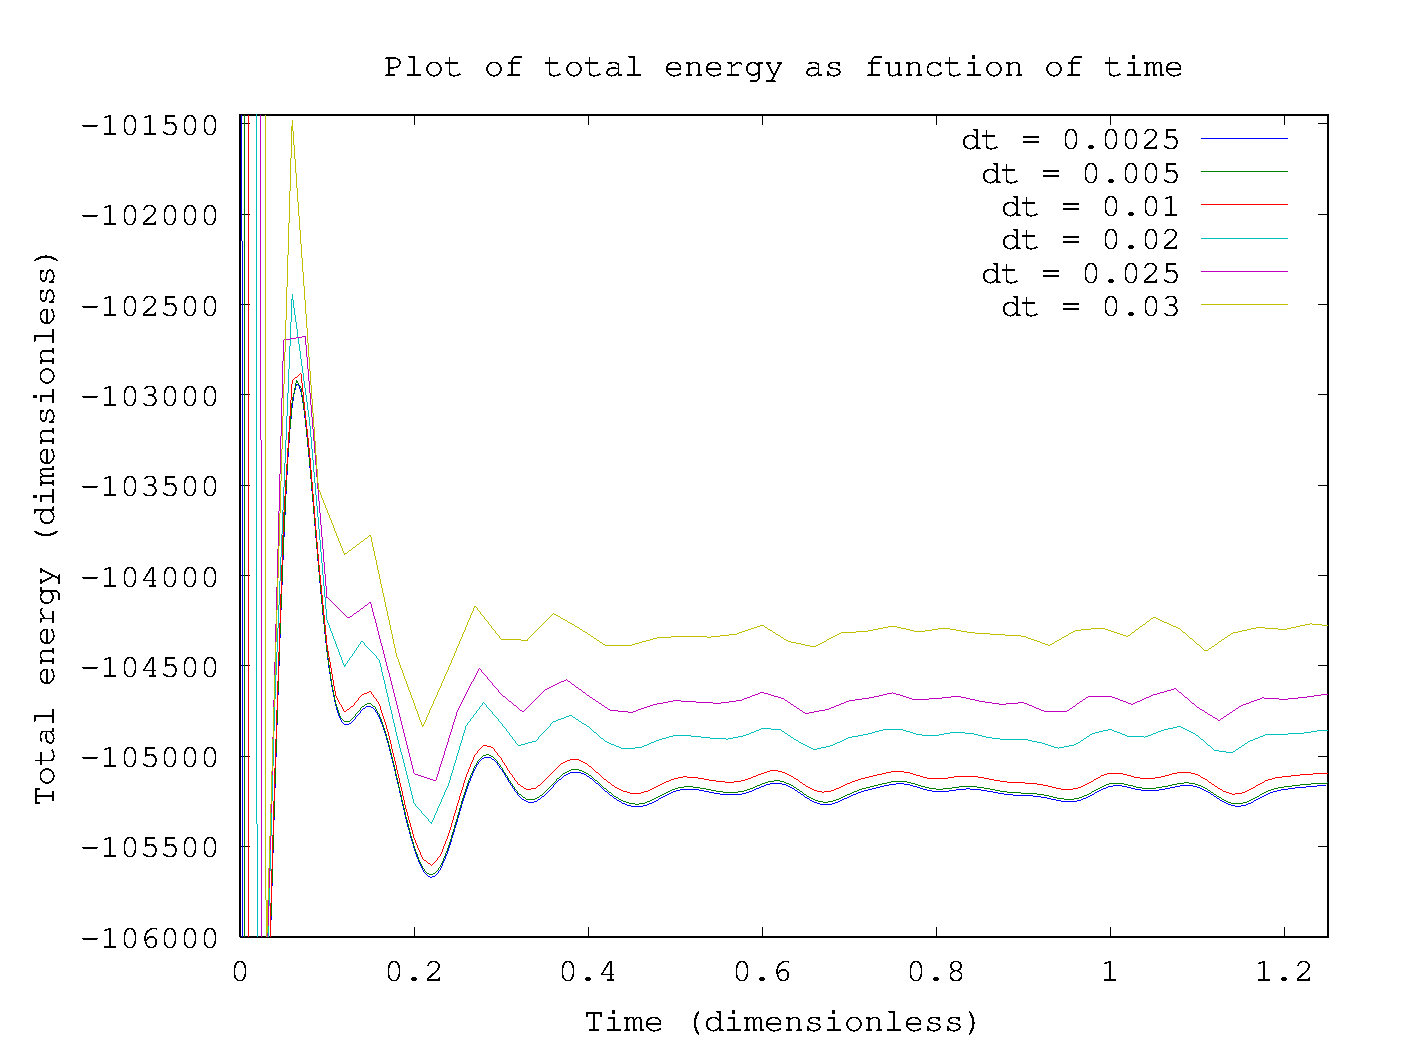
\includegraphics[width =.70\textwidth]{bilder/j_plot01.eps}
    \parbox{4in} {
        \caption{
            \small{
                Plot of the total internal energy of a 12x12x12 system of fcc cells (6912 atoms), with $a = 5.260$ \AA, for 500 timesteps. The system was initialized with normal distribution of velocities, with $\sigma'_v = \sqrt{T'}$ and $T' = 100$ K$/T_0$.
            }
            \label{fig:j}
        }
    }
\end{figure}

\subsection*{Temperature}
We can measure the temperature of the system using the average total kinetic energy, which according to the equipartition principle relates to the temperature as
\[
    \langle E_k \rangle \frac{3}{2}Nk_BT,
\]
where $N$ is the number of atoms and $T$ is the temperature. See Appendix for derivations of a dimensionless version of this. Using this relation we find the temperature, see figure \ref{fig:k} for plot of the temperature as function of time, and plots of the average temperature, for different system sizes. The simulations were started at $T' = 0.84$, but we see that they stabilize at approximately half this value. We see that the average temperature converges well at system sizes above approximately $N_C = 16$ (the number of fcc unit cells in each direction). This corresponds to 16384 atoms. We see that the fluctiations in temperature wary with system size, with the smaller systems having large fluctuations of $\pm 0.02$, and the smaller systems having fluctuations around $\pm 0.005$.
\begin{figure}
  \begin{center}
  \makebox[\textwidth] {
      \subfigure[] {
          \label{fig:k1}
          \includegraphics[width =.70\textwidth]{bilder/k_plot02.eps}
      }
      \subfigure[] {
          \label{fig:k2}
          \includegraphics[width =.70\textwidth]{bilder/k_plot03.eps}
      }
  }
  \parbox{5in} {
      \caption {
          \small {
              a) Plot of the (dimensionless) temperature as function of time, and b) plot of the average temperature of the system after equilibration, with standard deviation. We used different system sizes, all started in fcc configuration with $a = 5.260$ \AA. The simulation was run with $dt' = 0.01$. All systems was initialized with normal distribution of velocities, with $\sigma'_v = \sqrt{T'}$ and $T' = 100$ K$/T_0$. The averages were measured over 400 timesteps, after the system had equilibrated with 100 timesteps.
          }
          \label{fig:k}
      }
  }
  \end{center}
\end{figure}

\subsection*{Pressure}
We can measure the pressure using a method derived from the virial equation, which gives us
\[
    P = \rho k_B T + \frac{1}{3V}\sum_{i<j} \bvec F_{ij} \cdot \bvec r_{ij},
\]
where $V$ is the volume, and $\rho = V/N$ is the particle density. We compute the vector product inside the loops that calculate the force for efficiency, and the result can be seen in figure \ref{fig:l}. We see a clear indication of a first-order phase transition near $T' = 2.6$-2.7, where the pressure seems to be discontinous. We also noticed that we had to equilibrate the system for much longer when trying to get stable temperatures/pressures near this temperature (we only had to use 150 timesteps of $dt' = 0.005$ at most starting configurations, but the ones near $T' = 2.7$ required at least 500 timesteps).

It seems like we actually managed to make some kind of supercooled (or superheated) Argon state from the two points at $T' = 2.6$ and 2.4, which could make sense, seeing as the state out of those two that started with the highest temperature needed a lot more timesteps to equilibrate. See figure \ref{fig:l_eq} for plots of our attempts to equilibrate the system at temperatures near the phase 
transition.
\begin{figure}[h!]
    \centering
    \includegraphics[width =.70\textwidth]{bilder/l_plot01_2.eps}
    \parbox{4in} {
        \caption{
            \small{
                Plot of the pressure as function of temperature for a 12x12x12 system of fcc cells (6912 atoms), with $a = 5.260$ \AA, and timestep $dt' = 0.005$. The system was initialized with normally distributed velocities, equilibrated until convergence of both temperature and pressure, and then we collected data for the average for at least 350 cycles.
            }
            \label{fig:l}
        }
    }
\end{figure}

\begin{figure}[h!]
    \centering
    \includegraphics[width =.70\textwidth]{bilder/l_plot02.eps}
    \parbox{4in} {
        \caption{
            \small{
                Plot of the temperature as function of time for a 12x12x12 system of fcc cells (6912 atoms), with $a = 5.260$ \AA, and timestep $dt' = 0.005$. This is from our attempt to equilibrate the system near the phase transition at $T'\approx2.6$, used for the data collection for figure \ref{fig:l}. $T_0'$ indicates the temperature from which the standard deviation of the initial velocities is calculated.
            }
            \label{fig:l_eq}
        }
    }
\end{figure}

\subsection*{The diffusion constant}
We can find the self-diffusion of the atoms by measuring its position as function of time. The diffusion constant is related to the mean square displacement of all atoms
\[
    \langle r^2(t) \rangle = \frac{1}{N} \sum_{i=1}^N \left( \bvec r(t) - \bvec r_{\text{initial}} \right)^2,
\]
which we can relate to the diffusion constant in liquid through
\begin{align*}
    &\langle r^2(t) \rangle = 6Dt& &\text{when } t \rightarrow \infty&,
\end{align*}
where $D$ is the diffusion constant. See figure \ref{fig:n} for a plot of the diffusion constant for different temperatures. We see that $D$ depends approximately linearly on the temperature, in the temperature range we have measured.

\begin{figure}[h!]
    \centering
    \includegraphics[width =.70\textwidth]{bilder/n_plot01.eps}
    \parbox{4in} {
        \caption{
            \small{
                Plot of the diffusion constant as function of time for different temperatures, for a 12x12x12 system of Argon atoms. $T_0$ refers to the initial state of the system, where all particles had random, normally distributed velocities with standard deviation $\sigma_v = \sqrt{T_0}$. The system was in liquid phase for all plots.
            }
            \label{fig:n}
        }
    }
\end{figure}

\subsection*{The diffusion constant}
The radial distribution function $g(r)$ is the radial probability for finding another atom at a distance $r$ from an arbitrary atom. We have measured this by dividing the distance between atoms into intervals (bins), and looping over all atoms while finding the distances to all other atoms. The result can be seen in figure \ref{fig:o}, where we have averaged the function for 50 time-steps, and tested both a liquid and solid phase. We see that the distribution is very smooth in the liquid phase, as one would expect, and a bit jagged in the solid phase.

\begin{figure}
  \begin{center}
  \makebox[\textwidth] {
      \subfigure[] {
          \label{fig:o1}
          \includegraphics[width =.70\textwidth]{bilder/o_plot02.eps}
      }
      \subfigure[] {
          \label{fig:o2}
          \includegraphics[width =.70\textwidth]{bilder/o_plot01.eps}
      }
  }
  \parbox{5in} {
      \caption {
          \small {
              Plot of the radial distribution functiun $g(r)$ for a 12x12x12 Argon system in a) solid and b) liquid phase. The system was equilibrated before we collected data for the averages for 50 timesteps. The measurements were done by dividing the distance between atoms into intervals (bins), and looping over all atoms while checking the distance to all other atoms.
          }
          \label{fig:o}
      }
  }
  \end{center}
\end{figure}

\section*{Thermostats}
\subsection*{The Berendsen thermostat}
The Berendsen thermostat rescales the velocities of all atoms by a factor
\[
    \gamma = \sqrt{1 + \frac{\Delta t}{\tau} \left(\frac{T_{\text{bath}}}{T} - 1\right)},
\]
where $\tau$ is the relaxation time and $T_\text{bath}$ is the temperature of the external heat bath. The velocities is multiplied with this factor every timestep to simulate being in contact with the heat bath. By visualizing the motion of the atoms in Ovito we see that this thermostat doesn't have much impact on the observed motion of the atoms, as long as we keep the $\tau$ within 10-20 times the timestep. The atoms still seems to move very naturally and fluently.

\subsection*{The Andersen thermostat}
The Andersen thermostat simulates hard collisions between atoms inside the system with atoms in the heat bath. For all atoms we generate a random uniformly distributed number in $[0,1]$. If this number is smaller than $\frac{\Delta t}{\tau}$, the atom is given a new velocity. The new velocity is normally distributed with standard deviation $\sqrt{T'}$. Using this thermostat we see in the visualization that the atoms seems to behave a bit strange, similar to Brownian motion.

See figure \ref{fig:q} for a plot of the temperature as function of time using the two different thermostats. We see that the Berendsen thermostat gives a much smoother curve, just like we saw for the motion of the atoms, and that the Andersen thermostat gives a more jittery behaviour.

\begin{figure}[h!]
    \centering
    \includegraphics[width =.70\textwidth]{bilder/q_plot01.eps}
    \parbox{4in} {
        \caption{
            \small{
                Plot of temperature as function of time, for a 12x12x12 system, using two different thermostats to keep the temperature approximately constant.
            }
            \label{fig:q}
        }
    }
\end{figure}


\FloatBarrier
\section*{Appendix}
\subsection*{Some more dimensionless variables}
Here we have derived the dimensionless variables for some of the more complex equations used. First the standard deviation of the normal distribution for the initial velocities for the atoms
\begin{align*}
    \sigma_v &= \sqrt{\frac{k_BT}{m}} = \sqrt{\frac{k_BT'T_0}{m}} = \sqrt{\frac{\frac{\varepsilon}{T_0}T'T_0}{m}} = \sqrt{\frac{\varepsilon T'}{m}} \\
    &\sigma_v = \sigma_v'v_0 = \sigma_v' \frac{L_0}{t_0} \\
    &\Rightarrow \sigma_v' = \sigma_v \frac{t_0}{L_0} = \sqrt{T'} \sqrt{\frac{\varepsilon}{m}} \frac{\sigma}{\sigma \sqrt{m/\varepsilon}} \\
    &\phantom{\Rightarrow \sigma v'}= \sqrt{T'}.
\end{align*}

Then the Lennard-Jones potential itself
\begin{align*}
    U &= 4\varepsilon \left[\left(\frac{\sigma}{r}\right)^{12} - \left(\frac{\sigma}{r}\right)^6 \right] \\
    &= 4\varepsilon \left[\left(\frac{1}{r'}\right)^{12} - \left(\frac{1}{r'}\right)^6 \right] \\
    &= 4\varepsilon \left(1 - r'^6 \right)\frac{1}{r'^{12}} \\
    &\Rightarrow U' = \frac{U}{E_0} = \frac{U}{\varepsilon} = 4 \left(1 - r'^6 \right)\frac{1}{r'^{12}}.
\end{align*}

Then the kinetic energy
\begin{align*}
    K &= \frac{1}{2}mv^2 = \frac{1}{2}m_0v'^2v_0^2 \\
    &= \frac{1}{2}m_0v'^2 \left(\frac{L_0}{t_0}\right)^2 = \frac{1}{2}m_0v'^2 \left(\frac{\sigma}{\sigma\sqrt{m_0/\varepsilon}}\right)^2 \\
    &= \frac{1}{2}m_0v'^2 \frac{\varepsilon}{m_0} = \frac{1}{2}\varepsilon v'^2 \\
    &\Rightarrow K' = \frac{K}{E_0} = \frac{K}{\varepsilon} = \frac{1}{2} v'^2.
\end{align*}

The average of the total kinetic energy
\begin{align*}
    \langle E_k \rangle &= \frac{3}{2}Nk_B T = \frac{3}{2} Nk_B T'T_0 \\
    &= \frac{3}{2} Nk_B T'\frac{\varepsilon}{k_B} = \frac{3}{2} NT'\varepsilon \\
    \langle E_k \rangle &= \langle E_k'E_0 \rangle = \langle E_k' \rangle \varepsilon \\
    &\Rightarrow \langle E_k' \rangle = \frac{3}{2}NT'.
\end{align*}

The pressure
\begin{align*}
    P &= \frac{N}{V}k_B T + \frac{1}{3V} \sum_{i<j} \bvec F_{ij} \bvec r_{ij} \\
    &= \frac{N}{V'}T' \left(k_B \cdot \frac{\varepsilon}{k_B} \cdot \frac{1}{\sigma^3}\right) + \frac{1}{3V'} \left(\frac{1}{\sigma^3} \cdot \frac{\varepsilon}{\sigma} \cdot \sigma\right) \sum_{i<j} \bvec F'_{ij} \bvec r'_{ij} \\
    &= \frac{\varepsilon}{\sigma^3} \left(\frac{N}{V'}T' + \frac{1}{3V'} \sum_{i<j} \bvec F'_{ij} \bvec r'_{ij} \right) \\
\end{align*}
\begin{align*}
    P' &= P\frac{L_0^2}{F_0} = P\frac{\sigma^3}{\varepsilon} \\
    &= \frac{N}{V'}T' + \frac{1}{3V'} \sum_{i<j} \bvec F'_{ij} \bvec r'_{ij} \\
\end{align*}
